\section{Models}
\label{models}

So far we have motivated the need for better datasets and tasks to evaluate the
capabilities of machine reading models. We proceed by describing a number of
baselines, benchmarks and new models to evaluate against this paradigm.  We
define two simple baselines, the majority baseline ({\tt maximum frequency})
picks the entity most frequently observed in the context document, whereas the
exclusive majority ({\tt exclusive frequency}) chooses the entity most
frequently observed in the context but not observed in the query. The idea
behind this exclusion is that the placeholder is unlikely to be mentioned twice
in a single Cloze form query.

\subsection{Symbolic Matching Models}

Traditionally, a pipeline of NLP models has been used for attempting question
answering, that is models that make heavy use of linguistic annotation,
structured world knowledge and semantic parsing and similar NLP pipeline
outputs.
Building on these approaches, we define a number of NLP-centric models for our
machine reading task.

\paragraph{Frame-Semantic Parsing}

Frame-semantic parsing attempts to identify predicates and their arguments,
allowing models access to information about ``who did what to whom''. Naturally
this kind of annotation lends itself to being exploited for question answering.
We develop a benchmark that makes use of frame-semantic annotations
which we obtained by parsing our model with a state-of-the-art frame-semantic
parser \cite{Das:2013:SRL,Hermann:2014:SRL}. As the parser makes extensive use
of linguistic information we run these benchmarks on the unanonymised version of
our corpora. There is no significant advantage in this as the frame-semantic
approach used here does not possess the capability to generalise through a
language model beyond exploiting one during the parsing phase.
Thus, the key objective of evaluating machine comprehension abilities is
maintained. Extracting entity-predicate triples---denoted as
$(e_1,V,e_2)$---from both the query $q$ and context document $d$, we attempt to
resolve queries using a number of rules with an increasing recall/precision
trade-off as follows (Table \ref{tab:fsp}).

\begin{table}[h]\footnotesize
  \centering
  \begin{tabular}{@{}rllll@{}}
    \toprule
    & Strategy & Pattern $\in q$ & Pattern $\in d$ & Example (Cloze / Context) \\
    \midrule
    1 & Exact match & $(p,V,y)$ & $(\bm{x},V,y)$ & X loves Suse / \textbf{Kim} loves Suse \\
    2 & be.01.V match & $(p,\textit{be.01.V},y)$ & $(\bm{x},\textit{be.01.V},y)$ & X is president / \textbf{Mike} is president \\
    3 & Correct frame & $(p,V,y)$ & $(\bm{x},V,z)$ & X won Oscar / \textbf{Tom} won Academy Award \\
    4 & Permuted frame & $(p,V,y)$ & $(y,V,\bm{x})$ & X met Suse / Suse met \textbf{Tom} \\
    5 & Matching entity & $(p,V,y)$ & $(\bm{x},Z,y)$ & X likes candy / \textbf{Tom} loves candy \\
    6 & Back-off strategy & \multicolumn{3}{l}{\textit{Pick the most frequent entity from the context that doesn't appear in the query}} \\
    \bottomrule
  \end{tabular}
  \caption{Resolution strategies using PropBank triples. $\bm{x}$ denotes the
    entity proposed as answer, $V$ is a fully qualified PropBank frame (e.g.
    \textit{give.01.V}). Strategies are ordered by precedence and answers
    determined accordingly. This heuristic algorithm was iteratively
    tuned on the validation data set.
    \label{tab:fsp}
  }
\end{table}

For reasons of clarity, we pretend that all PropBank triples are of the form
$(e_1,V,e_2)$. In practice, we take the argument numberings of the parser into
account and only compare like with like, except in cases such as the permuted
frame rule, where ordering is relaxed. In the case of multiple possible answers
from a single rule, we randomly choose one.

\paragraph{Word Distance Benchmark}

We consider another baseline that relies on word distance measurements. Here, we
align the placeholder of the Cloze form question with each possible entity in
the context document and calculate a distance measure between the question and the
context around the aligned entity.
This score is calculated by summing the distances of every word in $q$
to their nearest aligned word in $d$, where alignment is defined by matching
words either directly or as aligned by the coreference system. We tune the
maximum penalty per word ($m=8$) on the validation data.

\subsection{Neural Network Models}
Neural networks have successfully been applied to a range of tasks in NLP.
This includes classification tasks such as sentiment analysis
\cite{Kalchbrenner:2014:DCNN} or POS tagging \cite{Collobert:2011:NLP}, as well
as generative problems such as language modelling or machine translation
\cite{Sutskever:2014:SSLNN}.
We propose three neural models for estimating the probability of word type $a$
from document $d$ answering query $q$:
\begin{align*}
  p(a | d, q) &\propto \exp \left(W(a) g(d,q) \right), \quad\text{s.t. } a \in
  V,
\end{align*}
where $V$ is the vocabulary\footnote{The vocabulary includes all the word types
  in the documents, questions, the entity maskers, and the question unknown
  entity marker.},
and $W(a)$ indexes row $a$ of weight matrix $W$ and through a slight abuse of
notation word types double as indexes. Note that we do not privilege entities or
variables, the model must learn to differentiate these in the input sequence.
The function $g(d,q)$ returns a vector embedding of a document and query pair.

\paragraph{The Deep LSTM Reader}
Long short-term memory (LSTM, \cite{Hochreiter:1997:LSTM}) networks have
recently seen considerable success in tasks such as machine translation and
language modelling \cite{Sutskever:2014:SSLNN}. When used for translation, Deep
LSTMs \cite{Graves:2012:SSLRNN} have shown a remarkable ability to embed long
sequences into a vector representation which contains enough information to
generate a full translation in another language. Our first neural model for
reading comprehension tests the ability of Deep LSTM encoders to handle
significantly longer sequences. We feed our documents one word at a time into
a Deep LSTM encoder, after a delimiter we then also feed the query into the
encoder. Alternatively we also experiment with processing the query then the
document. The result is that this model processes each document query pair as a
single long sequence. Given the embedded document and query the network
predicts which token in the document answers the query.

We employ a Deep LSTM cell with skip connections from each input $x(t)$ to every
hidden layer, and from every hidden layer to the output $y(t)$:
\begin{align*}
  x'(t,k) &= x(t)||y'(t,k-1), \quad\quad y(t) = y'(t,1) || \ldots || y'(t,K) \\
  \igate(t,k) &= \sigma\left(\wtmat{kx}{\igate} x'(t,k) + \wtmat{kh}{\igate} h(t-1,k) + \wtmat{k\state}{\igate} \state(t-1,k)  + b_{k\igate}\right)\\
  \fgate(t,k) &= \sigma\left(\wtmat{kx}{\fgate} x(t) + \wtmat{kh}{\fgate} h(t-1,k) + \wtmat{k\state}{\fgate} \state(t-1,k) + b_{k\fgate} \right)\\
  \state(t,k) &= \fgate(t,k) \state(t-1,k) + \igate(t,k) \tanh \left(\wtmat{kx}{\state} x'(t,k) + \wtmat{kh}{\state} h(t-1,k) + b_{k\state} \right) \\
  \ogate(t,k) &= \sigma\left(\wtmat{kx}{\ogate} x'(t,k) + \wtmat{kh}{\ogate} h(t-1,k) + \wtmat{k\state}{\ogate} \state(t,k) + b_{k\ogate}\right)\\
  h(t,k) &= \ogate(t,k) \tanh\left(\state(t,k)\right)\\
  y'(t,k) &= \wtmat{k}{y}h(t,k) + b_{ky}
\end{align*}
where $||$ indicates vector concatenation $h(t,k)$ is the hidden state for layer
$k$ at time $t$, and $\igate$, $\fgate$, $\ogate$ are the input, forget, and
output gates respectively.
Thus our Deep LSTM Reader is defined by $g^{\text{\tiny LSTM}}(d,q) = y(|d|+|q|)$ with input $x(t)$ the concatenation of $d$ and $q$ separated by the delimiter $|||$.

\paragraph{The Attentive Reader}

\newcommand{\attnIn}{m}
\newcommand{\attnU}{u}
\newcommand{\attnOver}{y}
\newcommand{\attnMix}{r}
\newcommand{\attnMid}{z}
\newcommand{\attnScore}{s}
\newcommand{\fwd}[1]{\overrightarrow{#1}}
\newcommand{\back}[1]{\overleftarrow{#1}}
\newcommand{\softmax}[2]{\frac{\exp\left(#1\right)}{#2}}

\begin{figure}
\centering
  \begin{subfigure}[b]{0.49\textwidth}
    \centering
    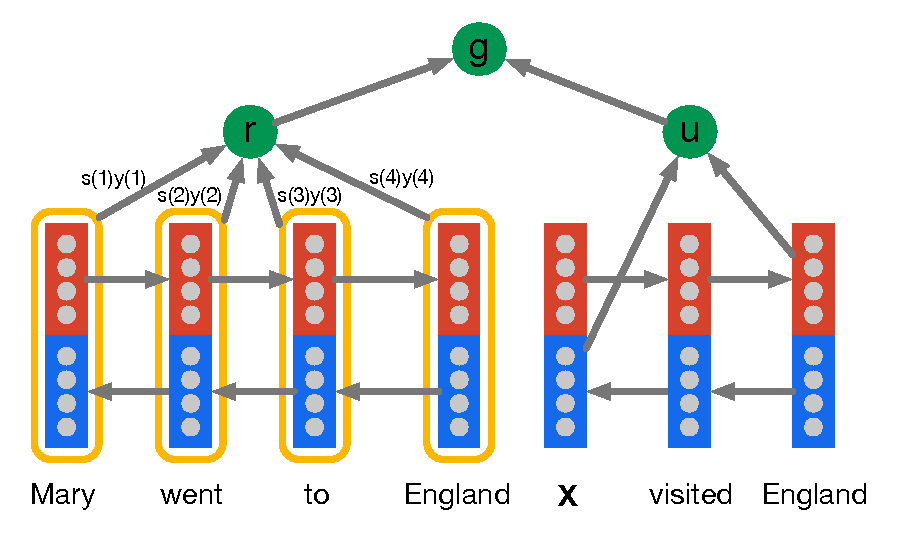
\includegraphics[scale=0.44]{figs/AttentiveReader.pdf}
    \caption{Attentive Reader.}
  \end{subfigure}
  \begin{subfigure}[b]{0.49\textwidth}
    \centering
    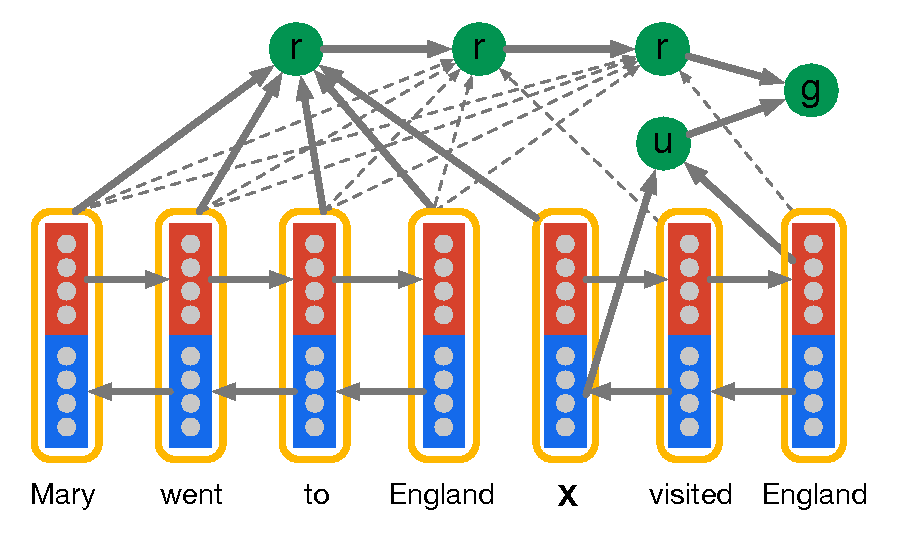
\includegraphics[scale=0.44]{figs/ImpatientReader.pdf}
    \caption{Impatient Reader.}
  \end{subfigure}
  \begin{subfigure}[b]{1.0\textwidth}
    \centering
    %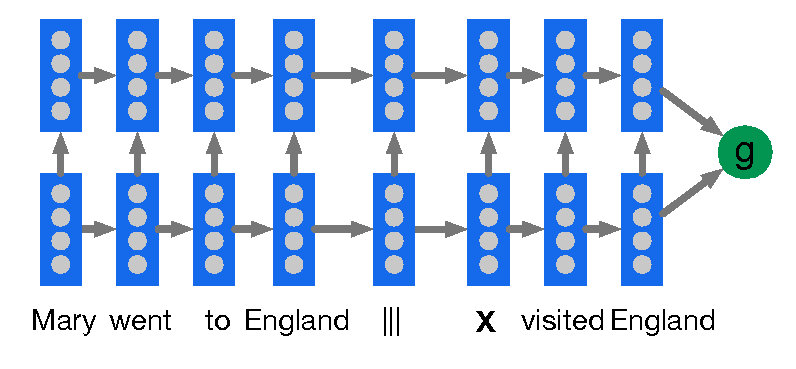
\includegraphics[scale=0.40]{figs/BiLSTM.pdf}
    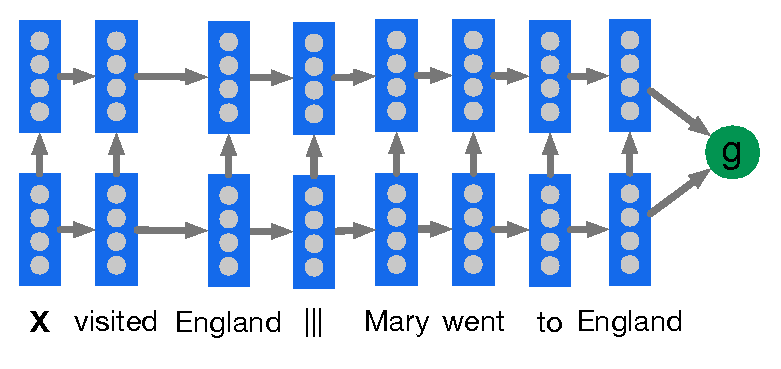
\includegraphics[scale=0.44]{figs/BiLSTMRev.pdf}
    \caption{A two layer Deep LSTM Reader with the question encoded before
             the document.}
  \end{subfigure}
  \caption{Document and query embedding models.}
\label{fig:models}
\end{figure}

The Deep LSTM Reader must propagate dependencies over long distances in order to
connect queries to their answers. The fixed width hidden vector forms a
bottleneck for this information flow that we propose to circumvent using an
attention mechanism inspired by recent results in translation and image
recognition \cite{Bahdanau:2014:NMT,Mnih:2014:RMVA}.
This attention model first encodes the document and the query using separate
bidirectional single layer LSTMs \cite{Graves:2012:SSLRNN}.

We denote the
outputs of the forward and backward LSTMs as $\fwd{y}(t)$ and $\back{y}(t)$
respectively.  The encoding $u$ of a query of length $|q|$ is formed by the
concatenation of the final forward and backward outputs,
$u = \fwd{y_q}(|q|)\,\, ||\,\, \back{y_q}(1).$

For the document the composite output for each token at position $t$ is,
$y_d(t) = \fwd{y_d}(t)\,\, ||\,\, \back{y_d}(t).$
The representation $r$ of the document $d$ is formed by a weighted sum of these
output vectors. These weights are interpreted as the degree to which the network
attends to a particular token in the document when answering the query:
\begin{align*}
  \attnIn(t)    &= \tanh\left(\wtmat{\attnOver}{\attnIn} \attnOver_d(t)
                   + \wtmat{\attnU}{\attnIn} \attnU\right),\\
  \attnScore(t) &\propto \exp \left(\mathrm{w}_{\attnIn\attnScore}^\intercal
                         \attnIn(t) \right),\\
  \attnMix   &= \attnOver_d \attnScore,
\end{align*}
where we are interpreting $y_d$ as a matrix with each column being the composite
representation $y_d(t)$ of document token $t$.
The variable $\attnScore(t)$ is the normalised attention at token $t$. Given
this attention score the embedding of the document $\attnMix$ is computed as the
weighted sum of the token embeddings.
The model is completed with the definition of the joint document and query
embedding via a non-linear combination:
\begin{align*}
  g^{\text{\tiny AR}}(d,q) = \tanh \left(\wtmat{\attnMix}{g} \attnMix
                             + \wtmat{\attnU}{g} \attnU \right).
\end{align*}

The Attentive Reader can be viewed as a generalisation of the application of
Memory Networks to question answering \cite{Weston:2014:MN}. That model employs
an attention mechanism at the sentence level where each sentence is represented
by a bag of embeddings. The Attentive Reader employs a finer grained token
level attention mechanism where the tokens are embedded given their entire
future and past context in the input document.

\paragraph{The Impatient Reader}
The Attentive Reader is able to focus on the passages of a context document
that are most likely to inform the answer to the query. We can go further by
equipping the model with the ability to reread from the document as each query
token is read. At each token $i$ of the query $q$ the model computes a document
representation vector $r(i)$ using the bidirectional embedding $y_q(i) =
\fwd{y_q}(i)\,\, ||\,\, \back{y_q}(i)$:
\begin{align*}
  \attnIn(i, t)   &= \tanh\left(\wtmat{d}{\attnIn} \attnOver_d(t)
                   + \wtmat{\attnMix}{\attnIn} \attnMix(i-1)
                   + \wtmat{q}{\attnIn} y_q(i) \right)
                , \quad 1 \leq i \leq |q|,  \\
  \attnScore(i,t) &\propto \exp \left(\mathrm{w}_{\attnIn\attnScore}^\intercal
                   \attnIn(i,t) \right),\\
  \attnMix(0)     &= \mathbf{r_0}, \quad
                   \attnMix(i)     = \attnOver_d^\intercal \attnScore(i) +
                   \tanh\left(\wtmat{\attnMix}{\attnMix}\attnMix(i-1)\right)
  \quad 1 \leq i \leq |q|.
\end{align*}
The result is an attention mechanism that allows the model to recurrently
accumulate information from the document as it sees each query token, ultimately
outputting a final joint document query representation for the answer prediction,
\begin{align*}
  g^{\text{\tiny IR}}(d,q) = \tanh \left(\wtmat{\attnMix}{g} \attnMix(|q|) +
                             \wtmat{q}{g} \attnU \right).
\end{align*}
